% 1977 年江苏盐城地区初试卷第四题：圆 O 外一点 A 作两条切线 AC、AD，
% C、D 为切点，连接 CO 并延长交 AD 延长线于 B（按源卷第 1 页布局：C 在圆左上方，D、B 在下方切线上）
% 坐标推算：A=(0,0)，D=(4,0)，B=(9,0)（AD=4，DB=5）；由 C、O、B 共线与 OD⊥AB 解得
% 半径 r=sqrt(80/13)≈2.481，O=(4,2.481)，C≈(1.778,3.583)
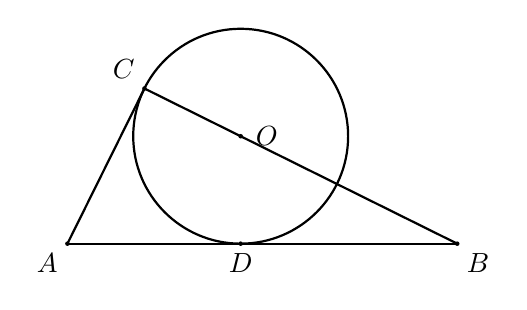
\begin{tikzpicture}[scale=0.55]
  \coordinate (A) at (0,0);
  \coordinate (D) at (4,0);
  \coordinate (B) at (9,0);
  \coordinate (O) at (4,2.481);
  \coordinate (C) at (1.778,3.583);
  \draw[thick] (O) circle (2.481);
  \draw[thick] (A) -- (B);
  \draw[thick] (A) -- (C);
  \draw[thick] (C) -- (B);
  \fill (O) circle (1.5pt) node[right=2pt] {$O$};
  \fill (A) circle (1.5pt) node[below left] {$A$};
  \fill (D) circle (1.5pt) node[below] {$D$};
  \fill (B) circle (1.5pt) node[below right] {$B$};
  \fill (C) circle (1.5pt) node[above left] {$C$};
\end{tikzpicture}
